% Options for packages loaded elsewhere
\PassOptionsToPackage{unicode}{hyperref}
\PassOptionsToPackage{hyphens}{url}
%
\documentclass[
]{book}
\usepackage{amsmath,amssymb}
\usepackage{lmodern}
\usepackage{ifxetex,ifluatex}
\ifnum 0\ifxetex 1\fi\ifluatex 1\fi=0 % if pdftex
  \usepackage[T1]{fontenc}
  \usepackage[utf8]{inputenc}
  \usepackage{textcomp} % provide euro and other symbols
\else % if luatex or xetex
  \usepackage{unicode-math}
  \defaultfontfeatures{Scale=MatchLowercase}
  \defaultfontfeatures[\rmfamily]{Ligatures=TeX,Scale=1}
\fi
% Use upquote if available, for straight quotes in verbatim environments
\IfFileExists{upquote.sty}{\usepackage{upquote}}{}
\IfFileExists{microtype.sty}{% use microtype if available
  \usepackage[]{microtype}
  \UseMicrotypeSet[protrusion]{basicmath} % disable protrusion for tt fonts
}{}
\makeatletter
\@ifundefined{KOMAClassName}{% if non-KOMA class
  \IfFileExists{parskip.sty}{%
    \usepackage{parskip}
  }{% else
    \setlength{\parindent}{0pt}
    \setlength{\parskip}{6pt plus 2pt minus 1pt}}
}{% if KOMA class
  \KOMAoptions{parskip=half}}
\makeatother
\usepackage{xcolor}
\IfFileExists{xurl.sty}{\usepackage{xurl}}{} % add URL line breaks if available
\IfFileExists{bookmark.sty}{\usepackage{bookmark}}{\usepackage{hyperref}}
\hypersetup{
  pdftitle={Deep learning tackles single-cell analysis - A survey of deep learning for scRNA-seq analysis},
  pdfauthor={Mario Flores, Zhentao Liu, Tinghe Zhang, Md Musaddaqui Hasib, Yu-Chiao Chiu, Zhenqing Ye, Karla Paniagua, Sumin Jo, Jianqiu Zhang, Shou-Jiang Gao, Yufang Jin, Yidong Chen, and Yufei Huang},
  hidelinks,
  pdfcreator={LaTeX via pandoc}}
\urlstyle{same} % disable monospaced font for URLs
\usepackage{longtable,booktabs,array}
\usepackage{calc} % for calculating minipage widths
% Correct order of tables after \paragraph or \subparagraph
\usepackage{etoolbox}
\makeatletter
\patchcmd\longtable{\par}{\if@noskipsec\mbox{}\fi\par}{}{}
\makeatother
% Allow footnotes in longtable head/foot
\IfFileExists{footnotehyper.sty}{\usepackage{footnotehyper}}{\usepackage{footnote}}
\makesavenoteenv{longtable}
\usepackage{graphicx}
\makeatletter
\def\maxwidth{\ifdim\Gin@nat@width>\linewidth\linewidth\else\Gin@nat@width\fi}
\def\maxheight{\ifdim\Gin@nat@height>\textheight\textheight\else\Gin@nat@height\fi}
\makeatother
% Scale images if necessary, so that they will not overflow the page
% margins by default, and it is still possible to overwrite the defaults
% using explicit options in \includegraphics[width, height, ...]{}
\setkeys{Gin}{width=\maxwidth,height=\maxheight,keepaspectratio}
% Set default figure placement to htbp
\makeatletter
\def\fps@figure{htbp}
\makeatother
\setlength{\emergencystretch}{3em} % prevent overfull lines
\providecommand{\tightlist}{%
  \setlength{\itemsep}{0pt}\setlength{\parskip}{0pt}}
\setcounter{secnumdepth}{5}
\usepackage{booktabs}
\ifluatex
  \usepackage{selnolig}  % disable illegal ligatures
\fi
\usepackage[]{natbib}
\bibliographystyle{apalike}

\title{Deep learning tackles single-cell analysis - A survey of deep learning for scRNA-seq analysis}
\author{\textbf{Mario Flores, Zhentao Liu, Tinghe Zhang, Md Musaddaqui Hasib, Yu-Chiao Chiu, Zhenqing Ye, Karla Paniagua, Sumin Jo, Jianqiu Zhang, Shou-Jiang Gao, Yufang Jin, Yidong Chen, and Yufei Huang}}
\date{2021-09-13}

\begin{document}
\maketitle

{
\setcounter{tocdepth}{1}
\tableofcontents
}
\begin{center}\rule{0.5\linewidth}{0.5pt}\end{center}

\hypertarget{front-matter}{%
\chapter*{Front Matter}\label{front-matter}}
\addcontentsline{toc}{chapter}{Front Matter}

\hypertarget{authors}{%
\subsection*{Authors}\label{authors}}
\addcontentsline{toc}{subsection}{Authors}

\textbf{Mario Flores\textsuperscript{1§}}, PhD, is an Assistant Professor in the Department of Electrical and Computer Engineering at the University of Texas at San Antonio, and joint program Faculty of Biomedical Engineering at the University of Texas Health San Antonio. Before joined ECE, he was a postdoctoral fellow at the National Center for Biotechnology Information of the National Institutes of Health from 2015 to 2019. His research focuses on DNA and RNA sequence methods, transcriptomics analysis, epigenetics, comparative genomics, and deep learning to study mechanisms of gene regulation, single-cell RNA-seq, and Natural Language Processing.

\textbf{Zhentao Liu1} is a PhD student in the Department of Electrical and Computer Engineering, the University of Texas at San Antonio. His research focuses on deep learning for cancer genomics and drug response prediction.

\textbf{Tinghe Zhang1} is a PhD student in the Department of Electrical and Computer Engineering, the University of Texas at San Antonio. His research focuses on deep learning for cancer genomics and drug response prediction.

\textbf{Md Musaddaqui Hasib1} is a PhD student in the Department of Electrical and Computer Engineering, the University of Texas at San Antonio. His research focuses on interpretable deep learning for cancer genomics.

\textbf{Yu-Chiao Chiu2}, PhD, is a postdoctoral fellow at the Greehey Children's Cancer Research Institute at the University of Texas Health San Antonio. His postdoctoral research is focused on developing deep learning models for pharmacogenomic studies.

\textbf{Zhenqing Ye2,3}, PhD, is an assistant professor in the Department of Population Health Sciences and the director of Computational Biology and Bioinformatics at Greehey Children's Cancer Research Institute at the University of Texas Health San Antonio. His research focuses on computational methods on next generation sequencing and single-cell RNA-seq data analysis.

\textbf{Karla Paniagua1}* is a PhD student in the Department of Electrical and Computer Engineering, the University of Texas at San Antonio. Her research focuses on \textasciitilde{}

\textbf{Sumin Jo1} is a PhD student in the Department of Electrical and Computer Engineering, the University of Texas at San Antonio. Her research focuses on m6A mRNA methylation and deep learning for biomedical applications.

\textbf{Jianqiu Zhang1}, PhD, is an Associate Professor in the Department of Electrical and Computer Engineering at the University of Texas at San Antonio. Her current research focuses on deep learning for biomedical applications such as m6A mRNA methylation.

\textbf{Shou-Jiang Gao4,6}, PhD, is a Professor in UPMC Hillman Cancer Center and Department of Microbiology and Molecular Genetics, University of Pittsburgh. His current research interests include Kaposi's sarcoma-associate herpesvirus (KSHV), AIDS-related malignancies, translational and cancer therapeutics, and systems biology.

\textbf{Yufang Jin1}, PhD, is a Professor in the Department of Electrical and Computer Engineering at the University of Texas at San Antonio. Her research focuses on mathematical modeling of cellular responses in immune systems, data-driven modeling and analysis of macrophage activations, and deep learning applications.

\textbf{Yidong Chen2,3}, PhD, is a Professor in the Department of Population Health Sciences and the director of Computational Biology and Bioinformatics at Greehey Children's Cancer Research Institute at the University of Texas Health San Antonio. His research interests include bioinformatics methods in next-generation sequencing technologies, integrative genomic data analysis, genetic data visualization and management, and machine learning in translational cancer research

\textbf{Yufei Huang5,6}, PhD, is a Professor in UPMC Hillman Cancer Center and Department of Medicine, School of Medicine, University of Pittsburgh. His current research interests include uncovering the functions of m6A mRNA methylation, cancer virology, and medical AI \& deep learning.

\hypertarget{corresponding-authors-mario-flores-mario.floresutsa.edu-yidong-chen-cheny8uthscsa.edu-and-yufei-huan-yuh119pitt.edu}{%
\subsubsection*{\texorpdfstring{\textbf{§Corresponding authors}: Mario Flores (\href{mailto:mario.flores@utsa.edu}{\nolinkurl{mario.flores@utsa.edu}}), Yidong Chen (\href{mailto:cheny8@uthscsa.edu}{\nolinkurl{cheny8@uthscsa.edu}}), and Yufei Huan (\href{mailto:yuh119@pitt.edu}{\nolinkurl{yuh119@pitt.edu}})}{§Corresponding authors: Mario Flores (mario.flores@utsa.edu), Yidong Chen (cheny8@uthscsa.edu), and Yufei Huan (yuh119@pitt.edu)}}\label{corresponding-authors-mario-flores-mario.floresutsa.edu-yidong-chen-cheny8uthscsa.edu-and-yufei-huan-yuh119pitt.edu}}
\addcontentsline{toc}{subsubsection}{\textbf{§Corresponding authors}: Mario Flores (\href{mailto:mario.flores@utsa.edu}{\nolinkurl{mario.flores@utsa.edu}}), Yidong Chen (\href{mailto:cheny8@uthscsa.edu}{\nolinkurl{cheny8@uthscsa.edu}}), and Yufei Huan (\href{mailto:yuh119@pitt.edu}{\nolinkurl{yuh119@pitt.edu}})}

\hypertarget{author-affiliations}{%
\subsubsection*{\texorpdfstring{\textbf{Author Affiliations}}{Author Affiliations}}\label{author-affiliations}}
\addcontentsline{toc}{subsubsection}{\textbf{Author Affiliations}}

1Department of Electrical and Computer Engineering, the University of Texas at San Antonio, San Antonio, TX 78249, USA

2Greehey Children's Cancer Research Institute, University of Texas Health San Antonio, San Antonio, TX 78229, USA

3Department of Population Health Sciences, University of Texas Health San Antonio, San Antonio, TX 78229, USA

4Department of Microbiology and Molecular Genetics, University of Pittsburgh, Pittsburgh, Pennsylvania, PA 15232, USA

5Department of Medicine, School of Medicine, University of Pittsburgh, PA 15232, USA

6UPMC Hillman Cancer Center, University of Pittsburgh, PA 15232, USA

\begin{center}\rule{0.5\linewidth}{0.5pt}\end{center}

\textbf{Book Maintainer}

Hello there :D

Any feedback and contributions will be appreciated.

Mail: \href{mailto:sumin.jo@utsa.edu}{\nolinkurl{sumin.jo@utsa.edu}}

Website: \href{https://github.com/Huang-AI4Medicine-Lab}{Huang-AI4Medicine-Lab}

\hypertarget{about-this-book}{%
\chapter*{About this book}\label{about-this-book}}
\addcontentsline{toc}{chapter}{About this book}

This book is full version of our research paper {[}Journal-Info-Here{]}.

\begin{quote}
\textbf{Keywords}
deep learning; single-cell RNA-seq; imputation; dimention reduction; clustering; batch correction; cell type identification; functional prediction; visualization
\end{quote}

\hypertarget{abstract}{%
\section*{Abstract}\label{abstract}}
\addcontentsline{toc}{section}{Abstract}

Since its selection as the method of the year in 2013, single-cell technologies have become mature enough to provide answers to complex research questions. However, together with the growth of single-cell profiling technologies, there has also been an increase of computational challenges to process the generated datasets. It's here that by effectively leveraging large data sets, Deep Learning (DL) is positioning as the first option for single-cell analyses. Here we provide a unified mathematical description of the DL methods used in single cell RNA sequencing (scRNA-Seq) followed with the survey of the most representative published DL algorithms for scRNA-Seq in the field.

\hypertarget{key-points}{%
\section*{Key Points}\label{key-points}}
\addcontentsline{toc}{section}{Key Points}

\begin{itemize}
\tightlist
\item
  Single cell RNA sequencing technology generate large collection of transcriptomic profiles of up to millions of cells, enabling biological investigation of hidden structures or cell types, predicting their effects or responses to treatment more precisely, or utilizing subpopulation to address unanswered hypotheses.
\item
  Current Deep Learning-based analysis approaches for single cell RNA seq data is systematically reviewed in this paper according to the challenge they address and their roles in the analysis pipeline.
\item
  A unified mathematical description of the surveyed DL models is presented and the specific model features were discussed when reviewing each approach.\\
\item
  A comprehensive summary of the evaluation metrics, comparision algorithms, and datasets by each approaches is presented.
\end{itemize}

\hypertarget{ch-1}{%
\chapter{Introduction}\label{ch-1}}

Single cell sequencing technology has been a rapidly developing area to study genomics, transcriptomics, proteomics, metabolomics, and cellular interactions at the single cell level for cell-type identification, tissue composition and reprogramming \citep{RN87, RN98}. Specifically, sequencing of the transcriptome of single cells, or single-cell RNA-sequencing (scRNA-seq), has become the dominant technology in many frontier research areas such as disease progression and drug discovery \citep{RN101, RN78, RN85}. One particular area where scRNA-seq has made a tangible impact is cancer, where scRNA-seq is becoming a powerful tool for understanding invasion, intratumor heterogeneity, metastasis, epigenetic alterations, detecting rare cancer stem cells, and assessing therapeutic response . Currently, scRNA-seq is applied to develop personalized therapeutic strategies that are potentially useful in cancer diagnosis, therapy resistance during cancer progression, and the survival of patients \citep{RN59, RN91}. The scRNA-seq has also been adopted to combat COVID-19 to elucidate how the innate and adaptive host immune system miscommunicates resulting in worsening immunopathology produced during this viral infection \citep{RN99}.

These studies have led to a massive amount of scRNA-seq data deposited to public databases such as Single Cell PORTAL, Single Cell Expression Atlas, PanglaoDB, and scRNASeqDB. Expressions of millions of cells from 18 species have been collected and deposited, waiting for further analysis. On the other hand, due to biological and technical factors, scRNA-seq data presents several analytical challenges related to its complex characteristics like missing expression values, high technical and biological variance, noise and sparse gene coverage, and elusive cell identities \citep{RN87}. These characteristics make it difficult to directly apply commonly used bulk RNA-seq data analysis techniques and have called for novel statistical approaches for scRNA-seq data cleaning and computational algorithms for data analysis and interpretation. To this end, specialized scRNA-seq analysis pipelines such as Seurat {[}9{]} and Scanpy {[}10{]}, along with a large collection of task-specific tools, have been developed to address the intricate technical and biological complexity of scRNA-seq data.

Recently, deep learning has demonstrated its significant advantages in natural language processing and speech and facial recognition with massive data. Such advantages have initiated the application of DL in scRNA-seq data analysis as a competitive alternative to conventional machine learning approaches for uncovering cell clustering {[}11, 12{]}, cell type identification {[}11, 13{]}, gene imputation {[}14-16{]}, and batch correction {[}17{]} in scRNA-seq analysis. Compared to conventional machine learning (ML) approaches, DL is more powerful in capturing complex features of high-dimensional scRNA-seq data. It is also more versatile, where a single model can be trained to address multiple tasks or adapted and transferred to different tasks. Moreover, the DL training scales more favorably with the number of cells in scRNA-seq data size, making it particularly attractive for handling the ever-increasing volume of single cell data. Indeed, the growing body of DL-based tools has demonstrated DL's exciting potential as a learning paradigm to significantly advance the tools we use to interrogate scRNA-seq data.

In this paper, we present a comprehensive review of the recent advances of DL methods for solving the present challenges in scRNA-seq data analysis (Table 1) from the quality control, normalization/batch effect reduction, dimension reduction, visualization, feature selection, and data interpretation by surveying deep learning papers published up to April 2021. In order to maintain high quality for this review, we choose not to include any (bio)archival papers, although a proportion of these manuscripts contain important new findings that would be published after completing their peer-reviewed process. Previous efforts to review the recent advances in machine learning methods focused on efficient integration of single cell data {[}18, 19{]}. A recent review of DL applications on single cell data has summarized 21 DL algorithms that might be deployed in single cell studies {[}20{]}. It also evaluated the clustering and data correction effect of these DL algorithms using 11 datasets.

In this review, we focus more on the DL algorithms with a much detailed explanation and comparison. Further, to better understand the relationship of each surveyed DL model with the overall scRNA-seq analysis pipeline, we organize the surveys according to the challenge they address and discuss these DL models following the analysis pipeline. A unified mathematical description of the surveyed DL models is presented and the specific model features are discussed when reviewing each method. This will also shed light on the modeling connections among the surveyed DL methods and the recognization of the uniqueness of each model. Besides the models, we also summarize the evaluation matrics of these DL algorithms and compare the tools that integrate these DL algorithms. Access to these DL algorithms with the original research results, available datasets used by these methods are also listed to demonstrate the advantages and utility of the DL algorithms. We envision that this survey will serve as an important information portal for learning the application of DL for scRNA-seq analysis and inspire innovative use of DL to address a broader range of new challenges in emerging multi-omics and spatial single-cell sequencing.

--\textgreater{}

\hypertarget{ch-2}{%
\chapter{Overview of scRNA-seq processing pipeline}\label{ch-2}}

Various scRNA-seq techniques (like SMART-seq, Drop-seq and 10X genomics sequencing {[}21, 22{]} are available nowadays with their sets of advantages and disadvantages. However, the data content and processing steps of different scRNA-seq techniques are quite standard and conventional. A typical scRNA-seq dataset consists of three files: genes quantified (gene IDs), cells quantified (cellular barcode) and a count matrix (number of cells × number of genes), irrespective of the technology or pipeline used. Conventionall, a series of essential steps are applied to these matrices for different analysis objectives as illustrated Fig. 1. These steps are:

\begin{figure}

{\centering 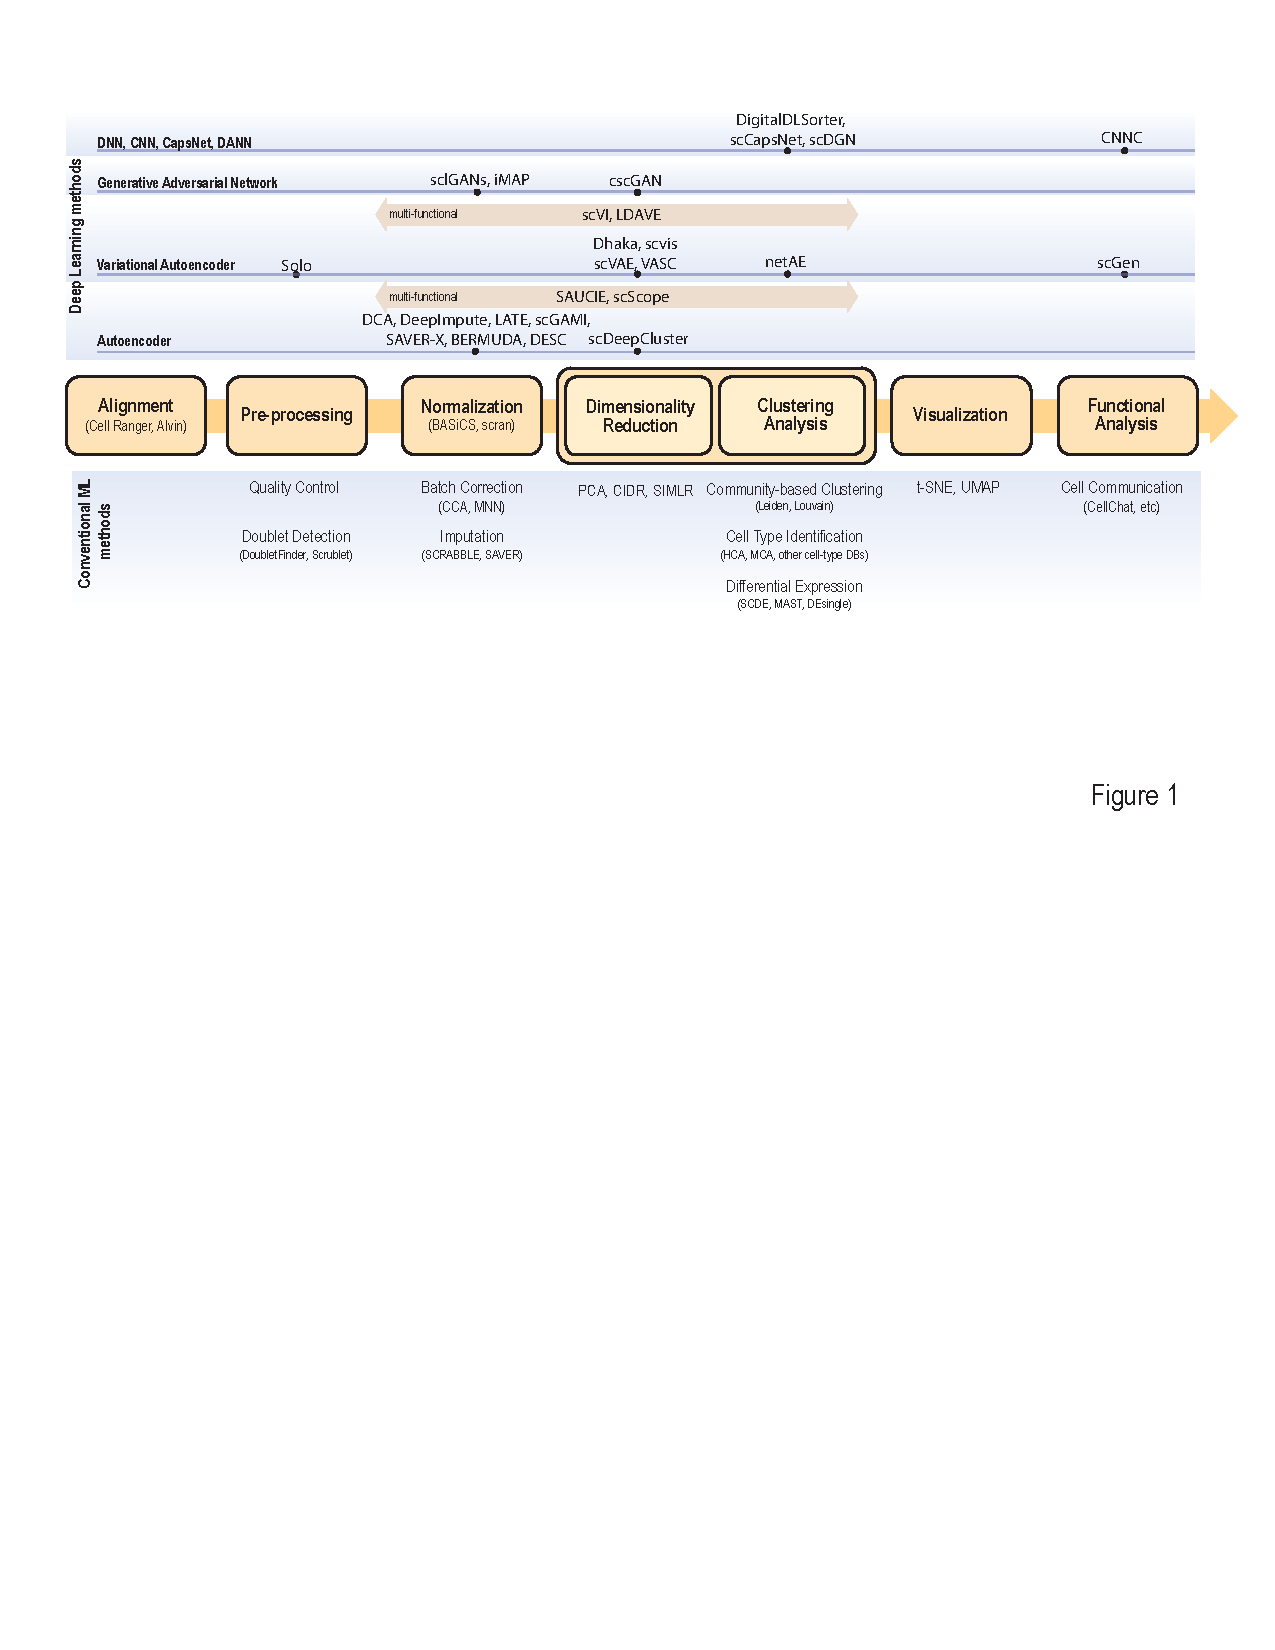
\includegraphics{Figures/Figure1} 

}

\caption{Single cell data analysis steps for both conventional ML methods (bottom) and DL methods (top). Depending on the input data and analysis objectives, major scRNA-se analysis steps are illustrated in the center flow chart. The convential ML approaches along with optional analysis modules are presented below each analysis step. Deep learning approaches are categorized as neural network models (DNN, CNN, CapsNet, and DANN), Generalive Adversarial Network (GAN), Variational Autoencoder, and Autoencoder. For each DL approach, optional algorithms are listed on top of each step in the pipeline.}\label{fig:Figure1}
\end{figure}

of the technology or pipeline used. A series of essential steps in scRNA-seq data processing pipeline and optional tools for each step with both ML and DL approaches are illustrated in Fig. 1.

With the advantage of identifying each cell and unique molecular identifiers (UMIs) for expressions of each gene in a single cell, scRNA-seq data are embedded with increased technical noise and biases {[}23{]}. Quality control (QC) is the first and the key step to filter out dead cells, double-cells, or cells with failed chemistry or other technical artifacts. The most commonly adopted three QC covariates include the number of counts (count depth) per barcode identifying each cell, the number of genes per barcode, and the fraction of counts from mitochondrial genes per barcode {[}24{]}.

Normalization is designed to eliminate imbalanced sampling, cell differentiation, viability, and many other factors. Approaches tailored for scRNA-seq have been developed including the Bayesian-based method coupled with spike-in, or BASiCS {[}25{]}, deconvolution approach, scran {[}26{]}, and sctransfrom in Seurat where regularized Negative Binomial regression was proposed {[}27{]}. Two important steps, batch correction and imputation, will be carried out if required by the analysis:
• Batch Correction is a common source of technical variation in high-throughput sequencing experiments due to variant experimental conditions such as technicians and experimental time, imposing a major challenge in scRNA-seq data analysis. Batch effect correction algorithms include detection of mutual nearest neighbors (MNNs) {[}28{]}, canonical correlation analysis (CCA) with Seurat {[}29{]}, and Hormony algorithm through cell-type representation {[}30{]}.
• Imputation step is necessary to handle high sparsity data matrix, due to missing value or dropout in scRNA-seq data analysis. Several tools have been developed to ``impute'' zero values in scRNA-seq data, such as SCRABBLE {[}31{]}, SAVER {[}32{]} and scImpute {[}33{]}.
Dimensionality reduction and visualization are essential steps to represent biological meaningful variation and high dimensionality with significantly reduced computational cost. Dimensionality reduction methods, such as PCA, are widely used in scRNA-seq data analysis to achieve that purpose. More advanced nonlinear approaches that preserve the topological structure and avoid overcrowding in lower dimension representation, such as LLE {[}34{]} (used in SLICER {[}35{]}), tSNE {[}36{]}, and UMAP {[}37{]} have also been developed and adopted as a standard in single-cell data visualization.

Clustering analysis is a key step to identify cell subpopulations or distinct cell types to unravel the extent of heterogeneity and their associated cell-type-specific markers. Unsupervised clustering is frequently used here to categorize cells into clusters by their similarity often taken the aforementioned dimensionality-reduced representations as input, such as community detection algorithm Louvain {[}38{]} and Leiden {[}39{]}, or data-driven dimensionality reduction followed with k-Means cluster by SIMLR {[}40{]}.

Feature selection is another important step in single-cell RNA-seq analysis is to select a subset of genes, or features, for cell-type identification and functional enrichment of each cluster. This step is achieved by differential expression analysis designed for scRNA-seq, such as MAST that used linear model fitting and likelihood ratio testing {[}41{]}; SCDE that adopted a Bayesian approach with a Negative Binomial model for gene expression and Poisson process for dropouts {[}42{]}, or DEsingle that utilized a Zero-Inflated Negative Binomial model to estimate the dropouts {[}43{]}.

Besides these key steps, downstream analysis can include cell type identification, coexpression analysis, prediction of perturbation response, where DL has also been applied. Other advanced analyses including trajectory inference and velocity and pseudotime analysis are not discussed here because most of the approaches on these topics are non-DL based.

  \bibliography{book.bib,packages.bib}

\end{document}
